\documentclass{beamer}
\usetheme{metropolis}
\usepackage[spanish]{babel}
\usepackage[utf8]{inputenc}
\usepackage{graphicx}
\usepackage{minted}
\setminted{
  style=colorful,
  linenos=true,
  fontsize=\small,
  tabsize=2,
  breaklines,
}
\usepackage{smartdiagram}
\usepackage{color}
\usepackage{subcaption}

\title{Estaciones satelitales}
\subtitle{Sistemas Inteligentes}
\author{Aarón Arias Pérez \\ Carlos Gallardo Polanco}
\institute{Escuela Superior de Ingeniería\\Universidad de Cádiz}
\date{11 de diciembre de 2017}

\begin{document}

\frame{\titlepage}

\section{¿Qué estrategias hemos elegido?}
\begin{frame}{Estrategias elegidas}
  \begin{center}
    \smartdiagram[bubble diagram]{PSR,
        Backtracking, Local Search, Simulated\\Annealing, Tabu\\Search, Genetic\\Algorithms, PSO}
  \end{center}
\end{frame}

\begin{frame}{Estrategias elegidas}
  \begin{center}
    \smartdiagram[bubble diagram]{PSR,
        \color{white}{Backtracking}, \color{white}{Local Search}, \textbf{Simulated}\\\textbf{Annealing}, \color{white}{Tabu}\\\color{white}{Search}, \textbf{Genetic}\\\textbf{Algorithms}, \color{white}{PSO}}
  \end{center}
\end{frame}

\section{Simulated Annealing}
\begin{frame}[fragile]{Simulated Annealing}
\begin{minted}{matlab}
function [best,value] = simulatedAnnealing(N,M,coordinates,T,T_limit,pcool)
  % T: Temperatura inicial
  % T_limit: Temperatura mínima
  current=randperm(N,M) % Representantes iniciales
  best=current; % La mejor es la inicial
  while (T>T_limit)
    RepToChange=current(randi(M));
    % Elegimos un representante aleatorio a cambiar
    new = random_sucessor(coordinates,current,RepToChange);
    % Nuevo conjunto de representantes aleatorio
\end{minted}
\end{frame}

\begin{frame}[fragile]
\begin{minted}[firstnumber=11]{matlab}
    deltaE = Fvalue(new,coordinates) - Fvalue(current,coordinates);
    if(deltaE<0) % Si la solución es mejor, se selecciona
      current = new;
      best = current;
    else
      if(exp(-deltaE/T)>rand(0,1)) % Acepta la solución de forma aleatoria
        current = new;
      end
    end
    T=cool(T,pcool);
  end
  value=Fvalue(best,coordinates);
end
\end{minted}
\end{frame}



\section{Algoritmos Genéticos}
\begin{frame}[fragile]{Algoritmos Genéticos}
\begin{minted}{matlab}
function [Pop,FitPop] = geneticAlgorithm(Pop, FitPop, coordinates, MAX_itera, Pcross, Pmut, cross, sel, rep)
  itera=1;
  while itera<=MAX_itera
    % RouletteWheel or Tournament
    parents = selection(FitPop,sel); % Selecciona los padres
    couples = match(parents,Pcross,itera); % Empareja los padres
\end{minted}
\end{frame}

\begin{frame}[fragile]
\begin{minted}[firstnumber=7]{matlab}
    if ~isempty(couples)
      % OX or PMX
      newPop = crossover(couples,Pop,cross); % Poblacion cruzada
    else
      newPop = Pop;
    end
    newPop = mutation(newPop,Pmut,size(coordinates,1)); % Población con mutaciones
    newFitPop = evaluatePopulation(newPop,coordinates);
    % generational or elitist
    [Pop,FitPop] = replace(Pop,newPop,FitPop,newFitPop,rep);
    itera=itera+1;
  end
end
\end{minted}
\end{frame}



\section{Comparativa SA y GA}
\begin{frame}{Simulated Annealing. Pruebas}
  \begin{center}
    \begin{figure}
      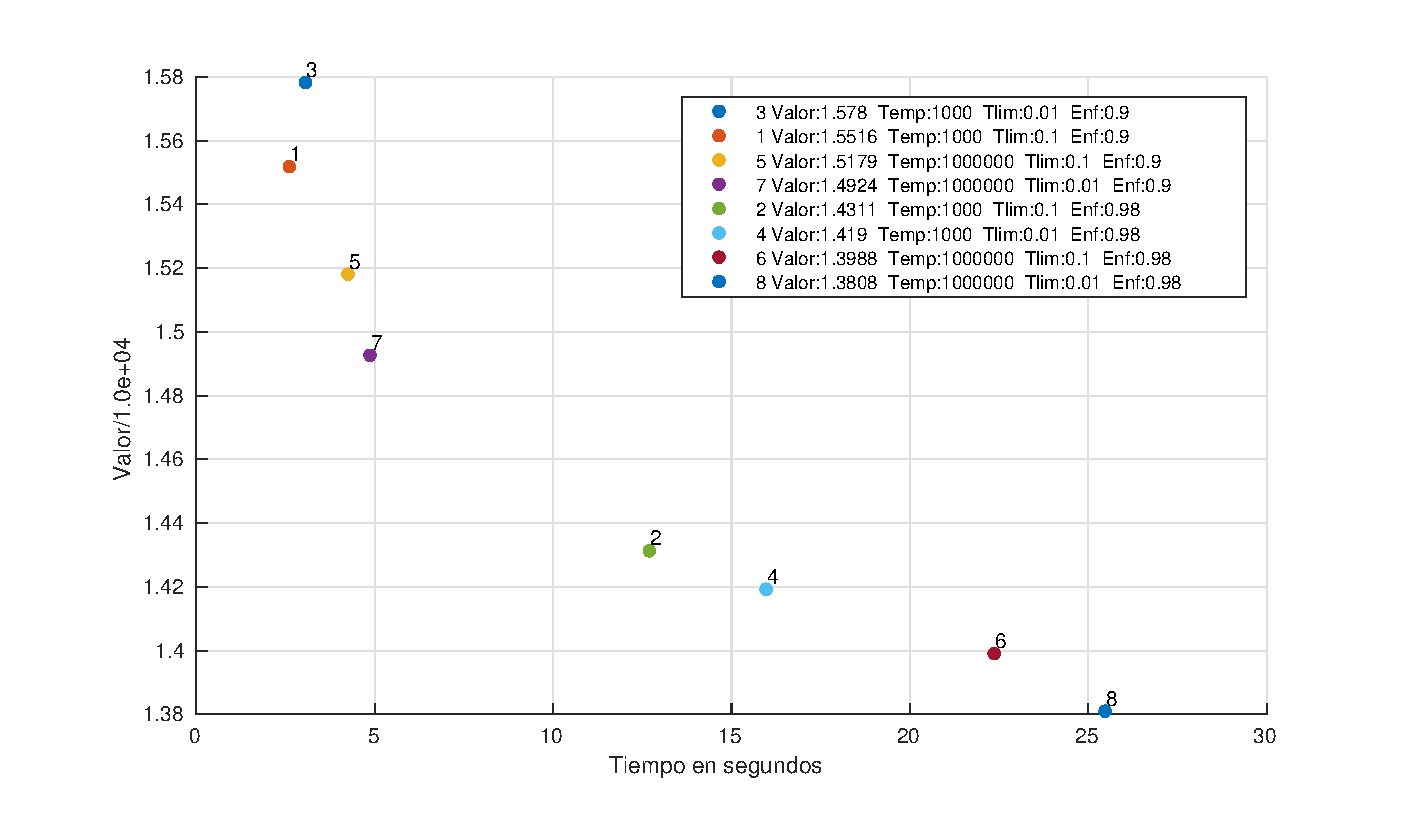
\includegraphics[scale=0.45]{../SA/statsSA.eps}
      \caption{Pruebas SA}
      \label{fig:statsSA}
    \end{figure}
  \end{center}
\end{frame}

\begin{frame}{Algoritmos Genéticos. Pruebas.}
  \begin{center}
    \begin{figure}
      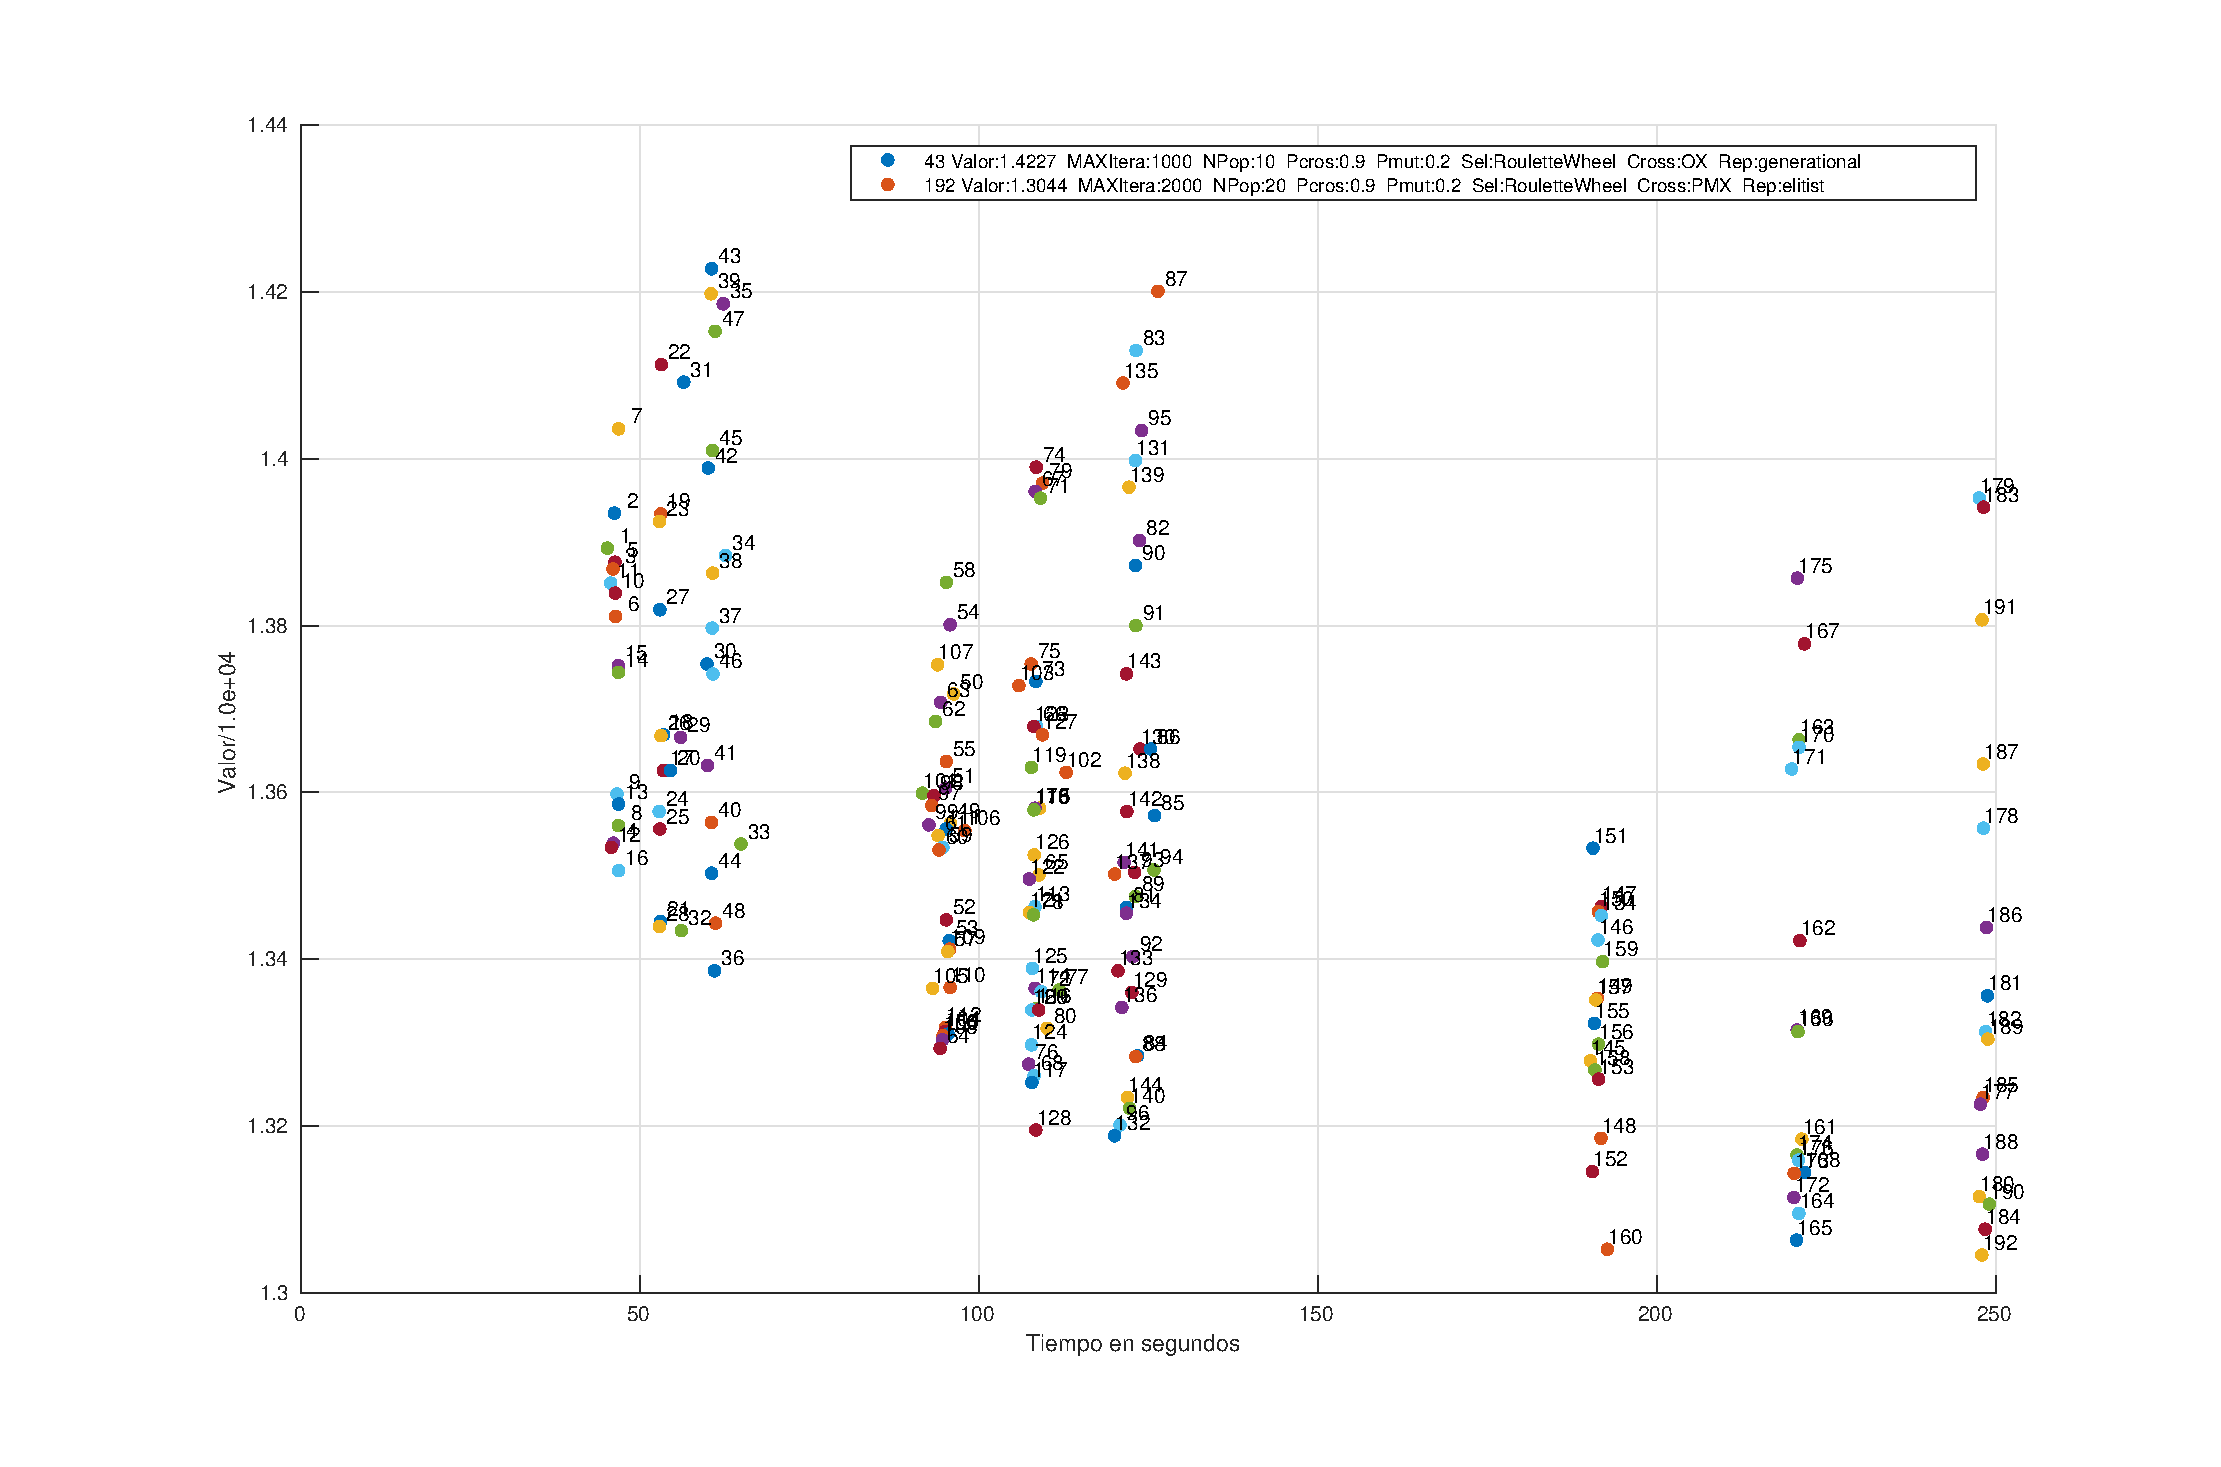
\includegraphics[scale=0.28]{../GA/statsGA.eps}
      \caption{Pruebas GA}
      \label{fig:statsGA}
    \end{figure}
  \end{center}
\end{frame}

\begin{frame}{Mapas}
  \begin{figure}
    \begin{subfigure}[b]{0.48\textwidth}
      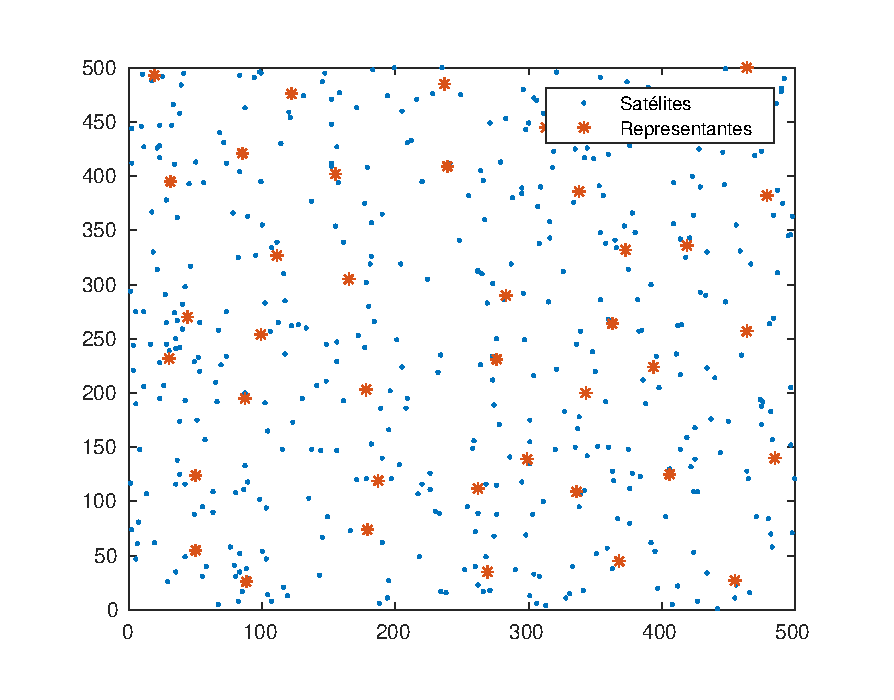
\includegraphics[width=\textwidth]{../SA/mapSA.eps}
      \caption{SA. Valor:1.3808e+04}
      \label{fig:mapSA}
    \end{subfigure}
    ~
    \begin{subfigure}[b]{0.48\textwidth}
      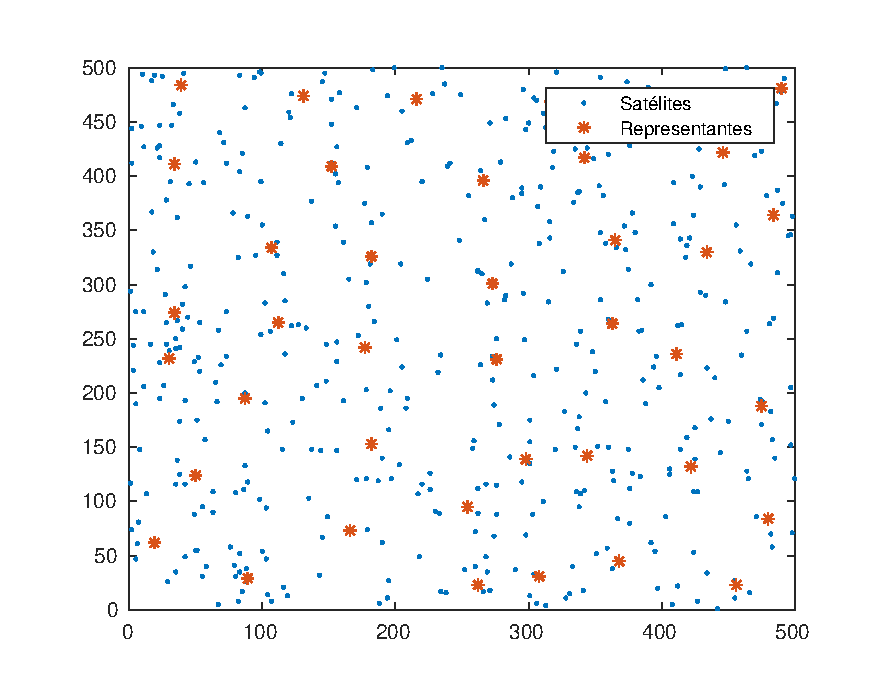
\includegraphics[width=\textwidth]{../GA/mapGA.eps}
      \caption{GA. Valor:1.3044e+04}
      \label{fig:mapGA}
    \end{subfigure}
    \caption{Mapas de los satélites}
    \label{fig:maps}
  \end{figure}
\end{frame}



\begin{frame}[standout]
  \huge{¿Preguntas?}
\end{frame}

\end{document}
